\begin{frame}
\frametitle{Feature engineering}
\emph{First-timers are often surprised by how {\bf little time in a machine learning project is spent actually doing machine learning}.
But it makes sense if you consider how time-consuming it is to gather data, integrate it, clean it and pre-process it, and how much {\bf trial and error can go into feature design}.
Also, machine learning is not a one-shot process of building a data set and running a learner, but rather an iterative process of running the learner, analyzing the results, modifying the data and/or the learner, and repeating.
Learning is often the quickest part of this, but that's because we've already mastered it pretty well!
{\bf Feature engineering is more difficult because it's domain-specific, while learners can be largely general-purpose.}
However, there is no sharp frontier between the two, and this is another reason {\bf the most useful learners are those that facilitate incorporating knowledge}.
}

\vspace{1cm}
\begin{tiny}
Domingos, Pedro. ``A few useful things to know about machine learning.'' Communications of the ACM 55, no. 10 (2012): 78-87.\par
\end{tiny}
\end{frame}

\begin{frame}
\frametitle{Region volumes}
\begin{columns}[c]
\column{0.33\textwidth}
Label propagation or other methods can be used to subdivide brain into regions.\par

\column{0.67\textwidth}
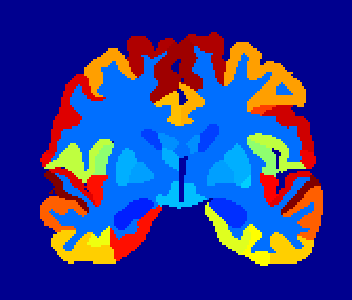
\includegraphics[width=\textwidth]{brain-regions}
\end{columns}
\end{frame}

\begin{frame}
\frametitle{Pixel values}
\begin{columns}[c]
\column{0.33\textwidth}
Raw pixel data could be another option.\par
Data needs to be ``spatially normalised'' (and possibly skull-stripped).\par
Results may not generalise well to data from other scanners.\par
\column{0.67\textwidth}
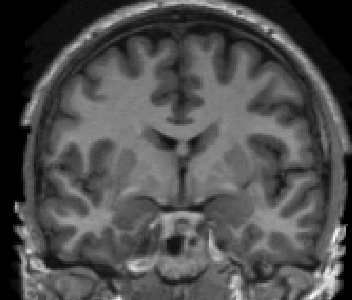
\includegraphics[width=\textwidth]{brain-raw}
\end{columns}
\end{frame}

\begin{frame}
\frametitle{Tissue maps}
\begin{columns}[c]
\column{0.33\textwidth}
Grey matter maps can work fairly well.\par
Data needs to be ``spatially normalised''.\par
Many neurological problems show up as grey matter atrophy.\par
\column{0.67\textwidth}
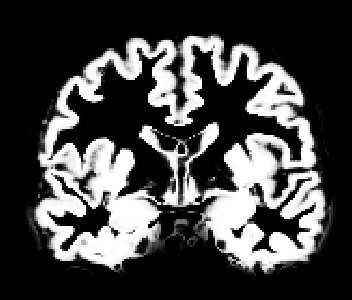
\includegraphics[width=\textwidth]{brain-GM}
\end{columns}
\end{frame}

\begin{frame}
\frametitle{Other features}
\begin{columns}[c]
\column{0.33\textwidth}
Other features include:
\begin{itemize}
\item Cortical thickness.
\item Shape features.
\item Principal / Independent component weights.
\item Lesion maps.
\item etc
\end{itemize}
\column{0.67\textwidth}
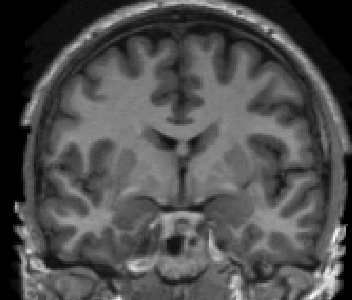
\includegraphics[width=\textwidth]{brain-raw}
\end{columns}
\end{frame}

